\documentclass{cmspaper}
\usepackage{graphicx}
\newcommand{\usedLumi}{1.1~fb$^{-1}$}
\begin{document}


\title{Upper limits for \usedLumi}

\begin{figure}[!htbp]
\begin{center}
   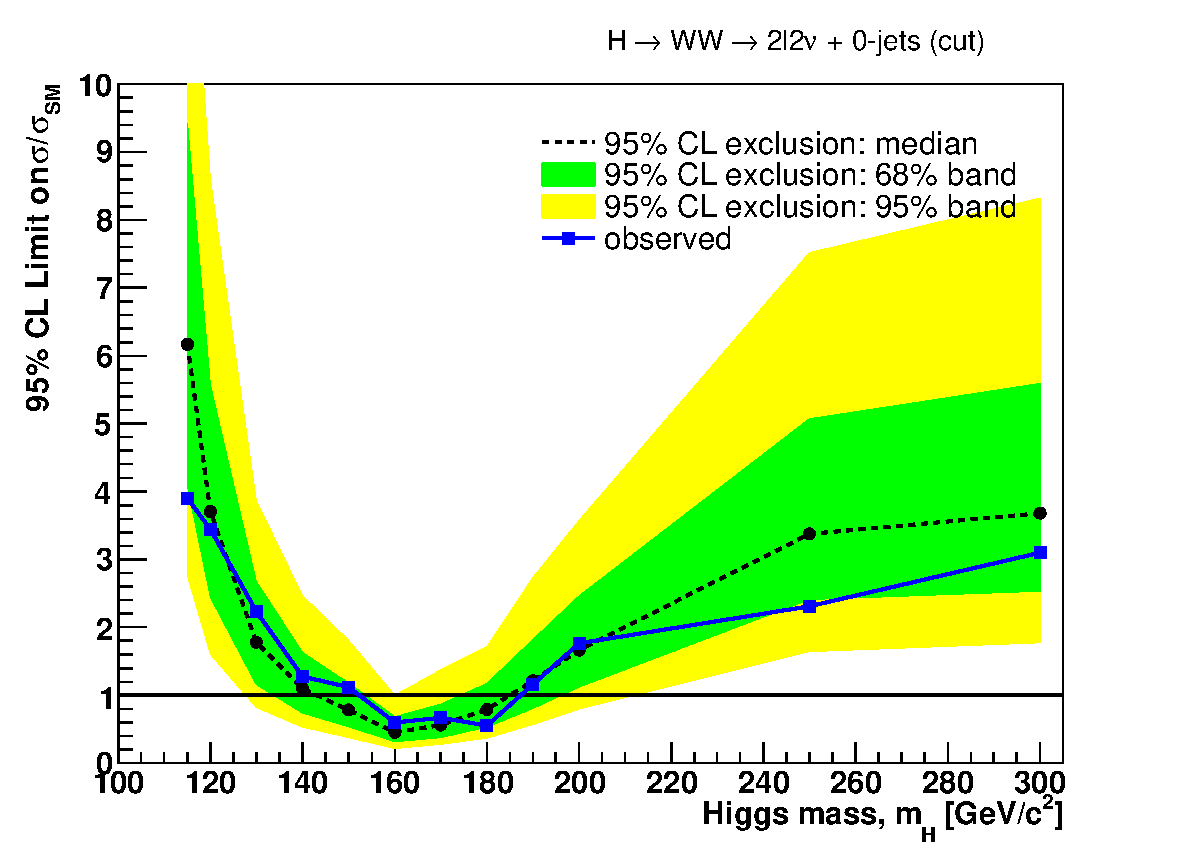
\includegraphics[width=0.49\textwidth]{eps_final/limits_0j_cut.pdf}
   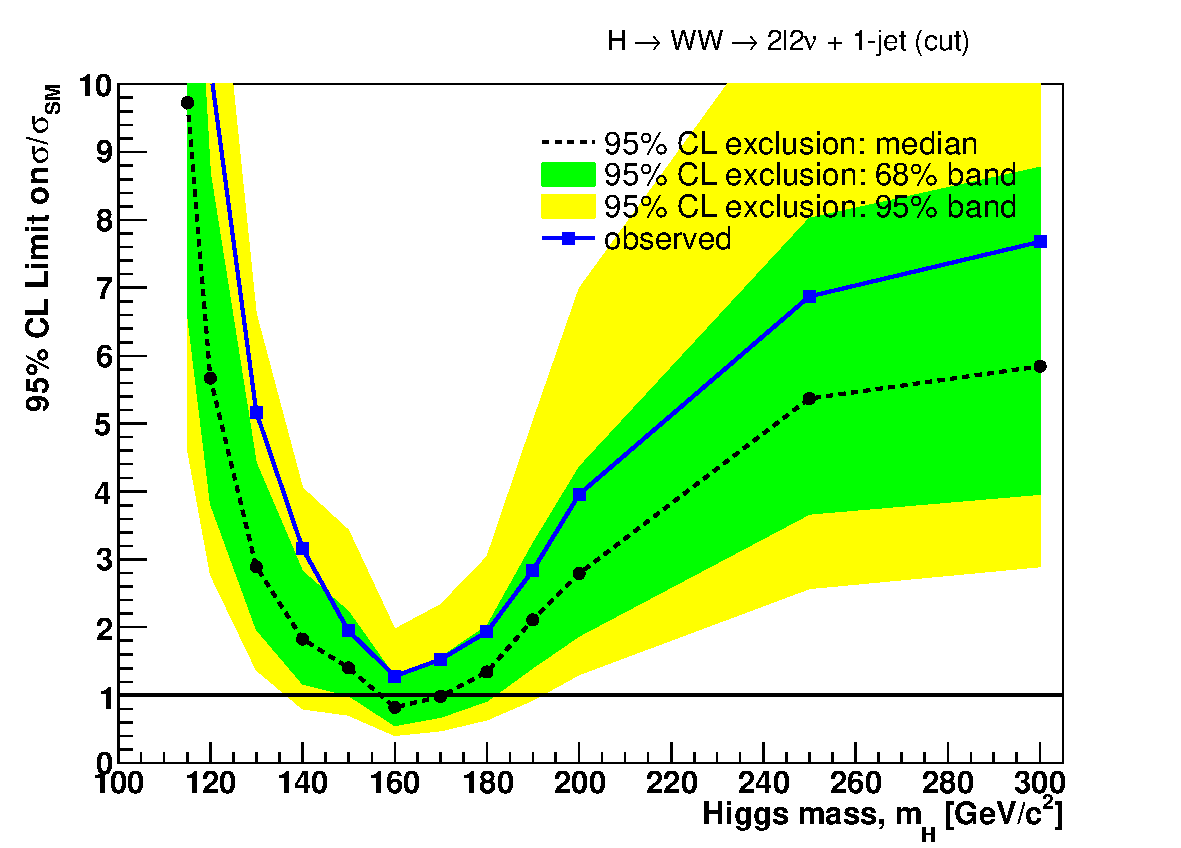
\includegraphics[width=0.49\textwidth]{eps_final/limits_1j_cut.pdf}
   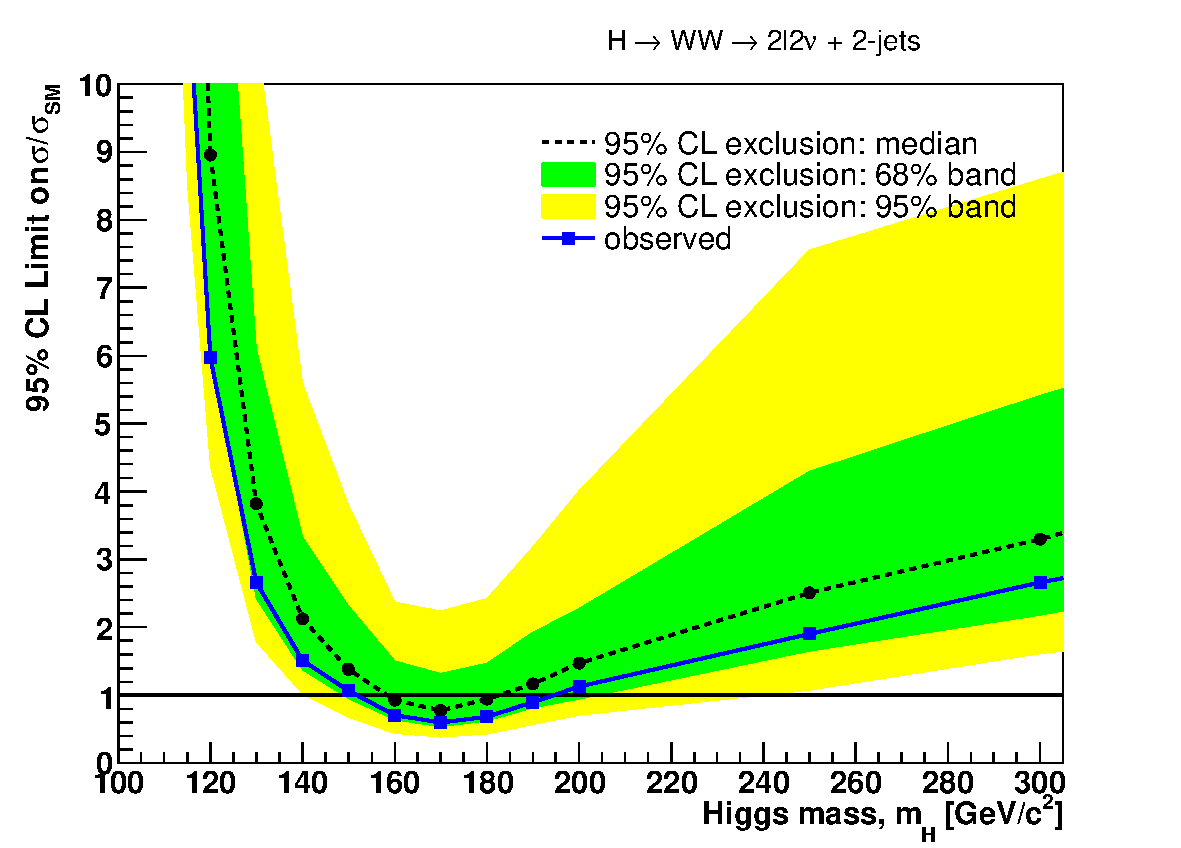
\includegraphics[width=0.49\textwidth]{eps_final/limits_2j_cut.pdf}
   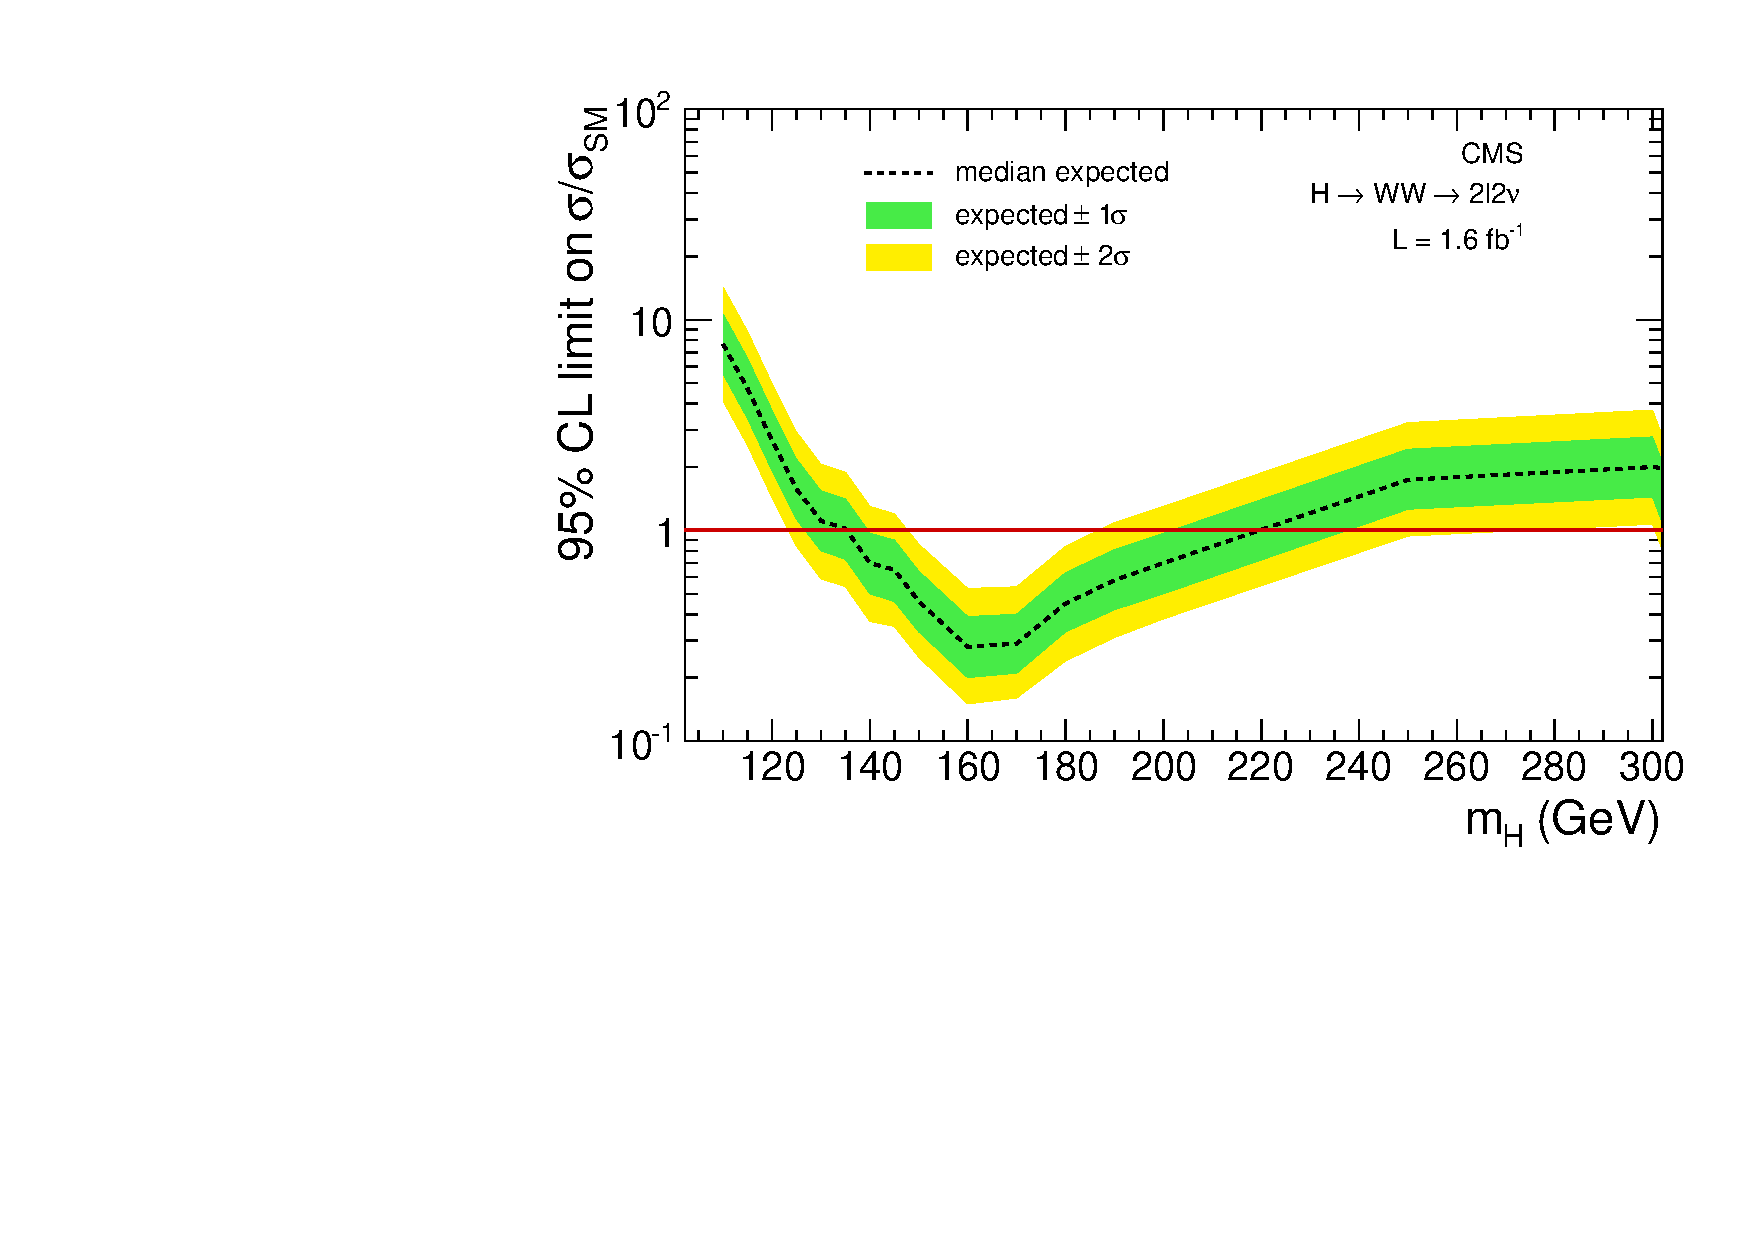
\includegraphics[width=0.49\textwidth]{eps_final/limits_nj_cut.pdf}
   \caption{Cut based analysis upper limits at 95\% C.L. for \usedLumi of data.}
\end{center}
\end{figure}

\begin{figure}[!htbp]
\begin{center}
   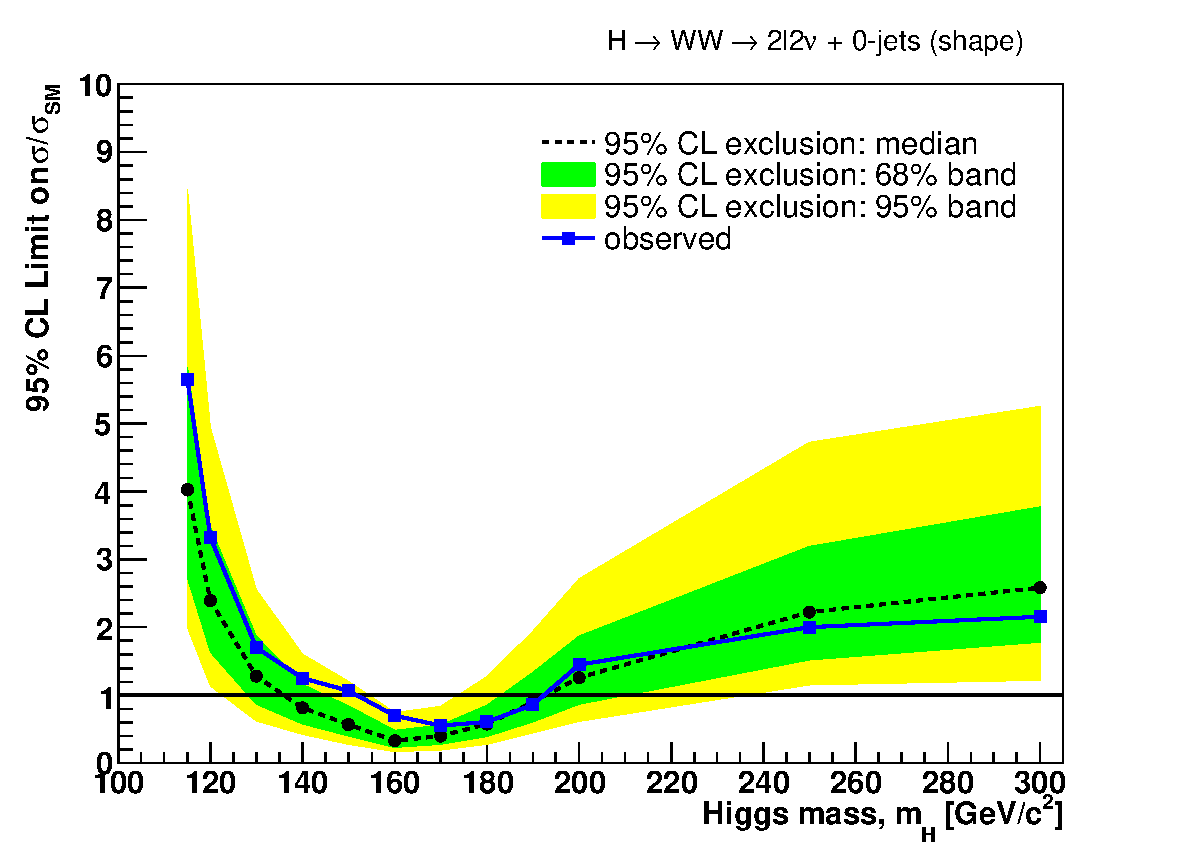
\includegraphics[width=0.49\textwidth]{eps_final/limits_0j_shape.pdf}
   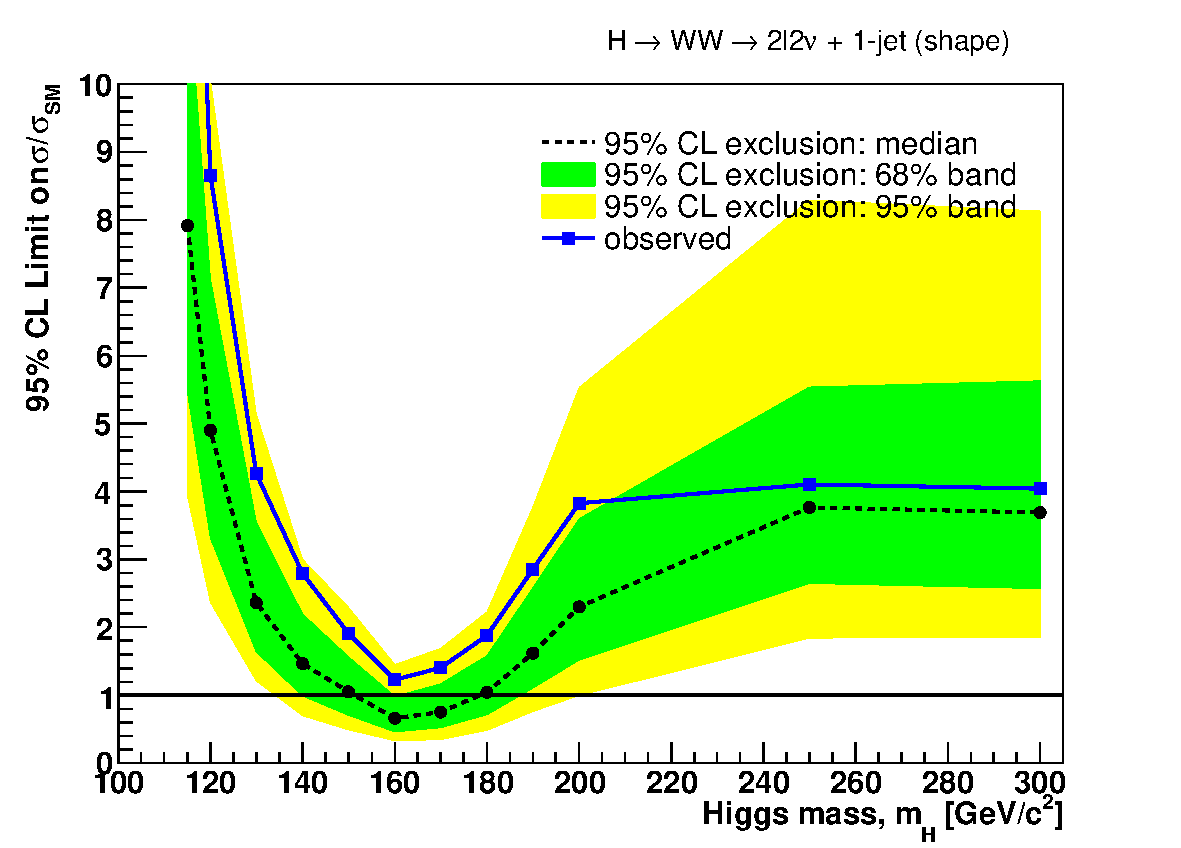
\includegraphics[width=0.49\textwidth]{eps_final/limits_1j_shape.pdf}
   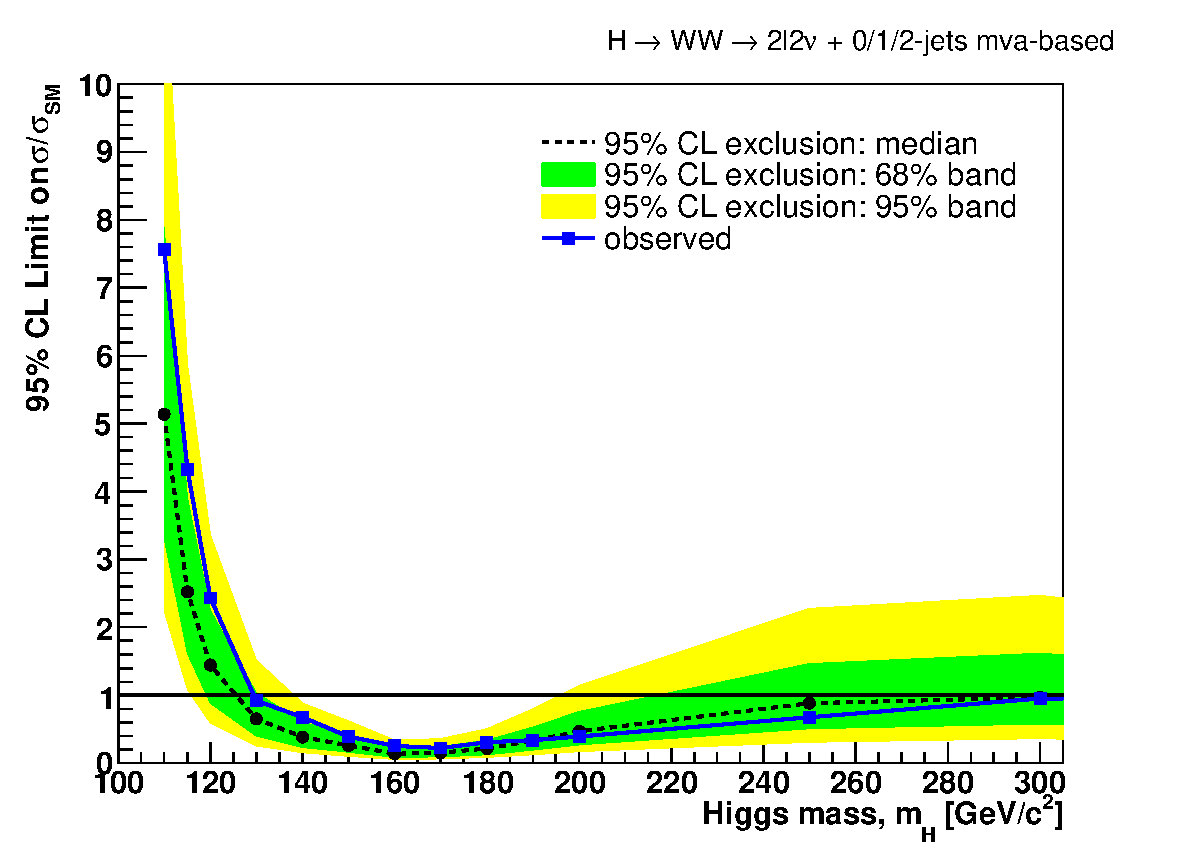
\includegraphics[width=0.49\textwidth]{eps_final/limits_nj_shape.pdf}
   \caption{Shape based analysis upper limits at 95\% C.L. for \usedLumi of data.}
\end{center}
\end{figure}


\begin{figure}[!htbp]
\begin{center}
   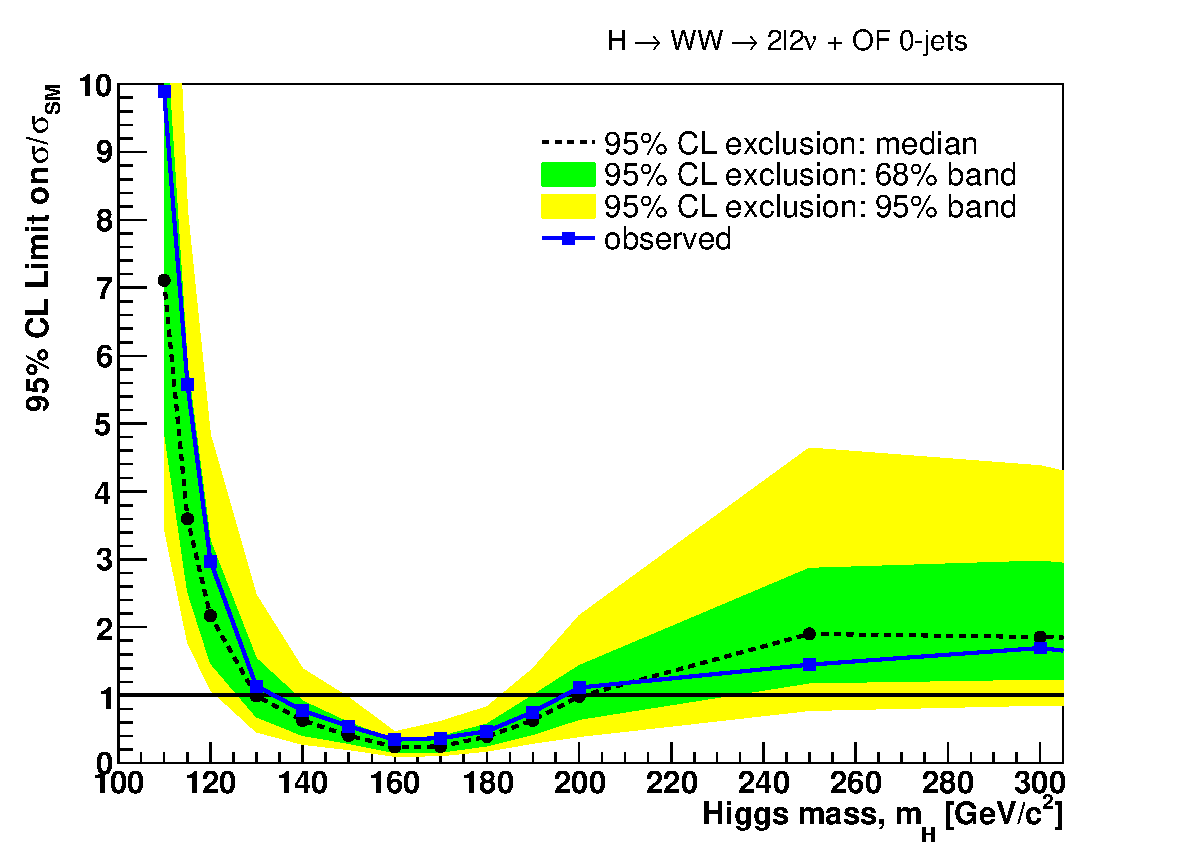
\includegraphics[width=0.49\textwidth]{eps_final/limits_of_0j_shape.pdf}
   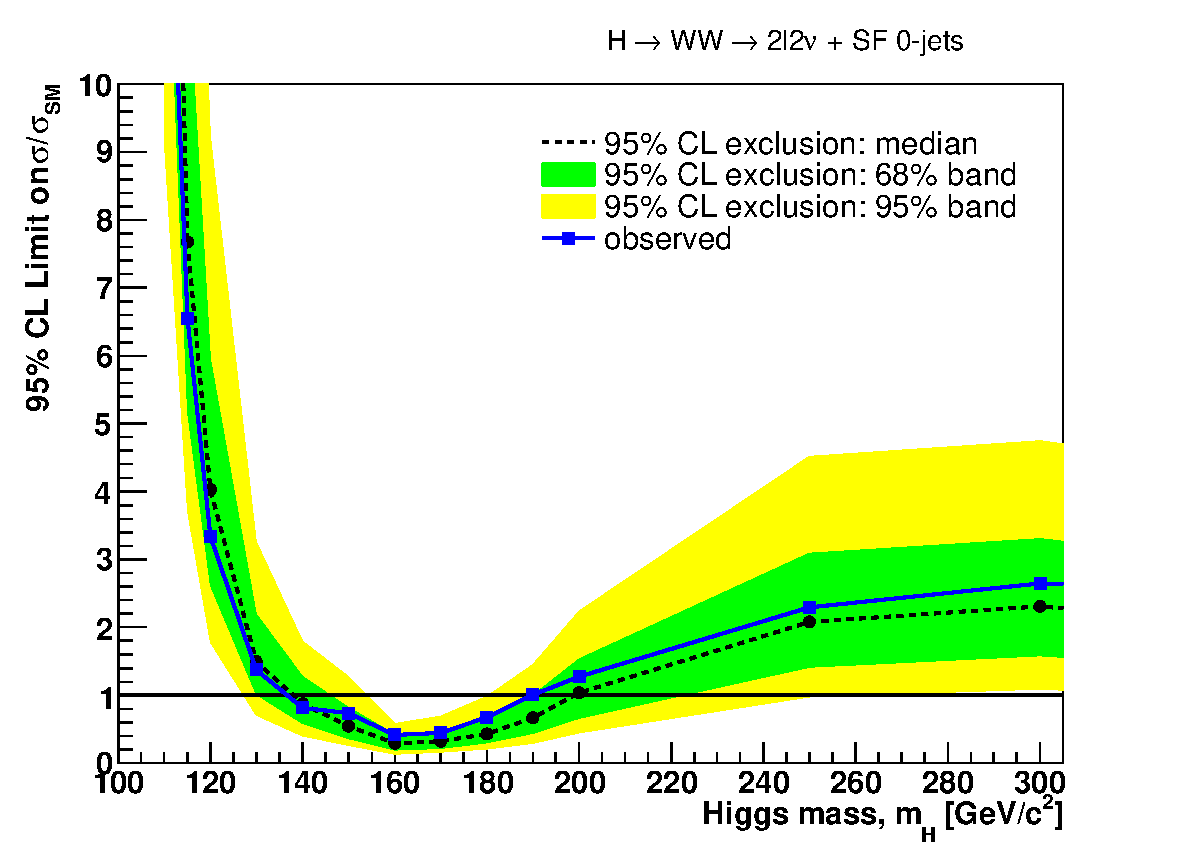
\includegraphics[width=0.49\textwidth]{eps_final/limits_sf_0j_shape.pdf}
   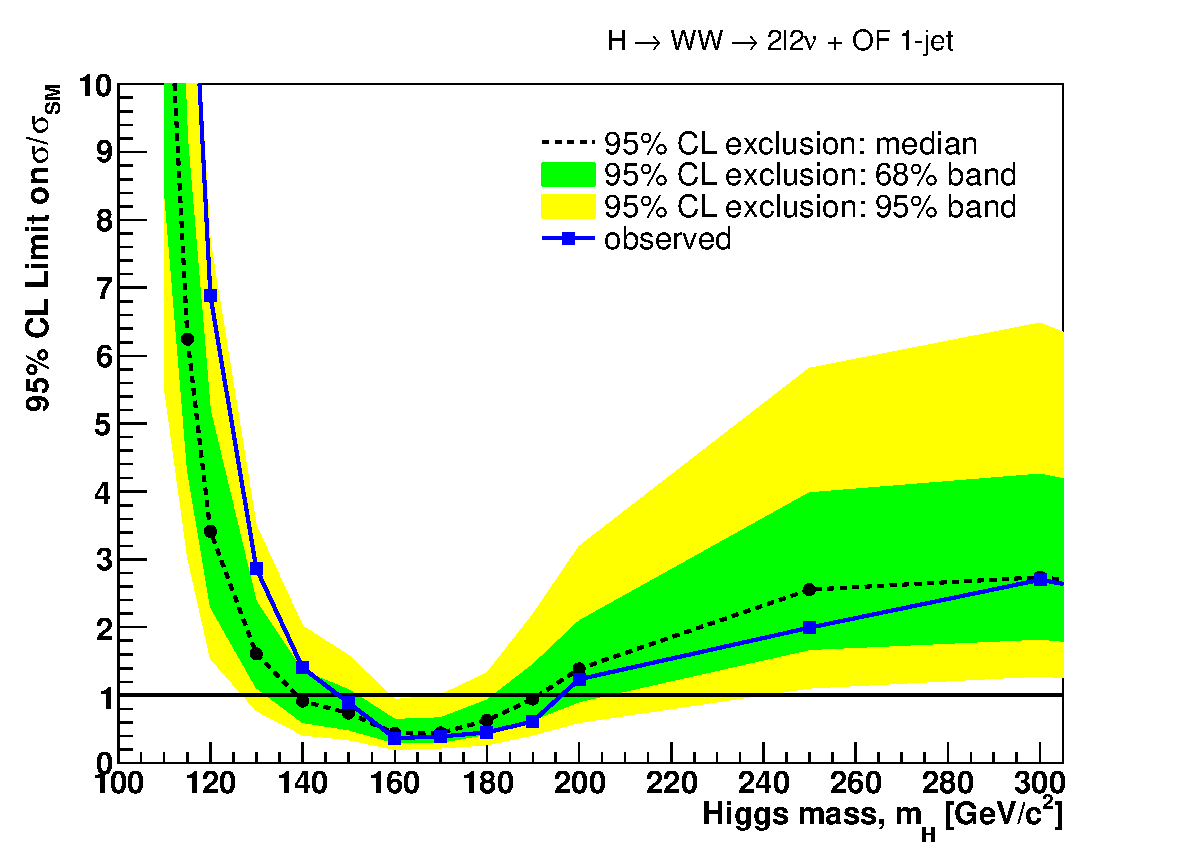
\includegraphics[width=0.49\textwidth]{eps_final/limits_of_1j_shape.pdf}
   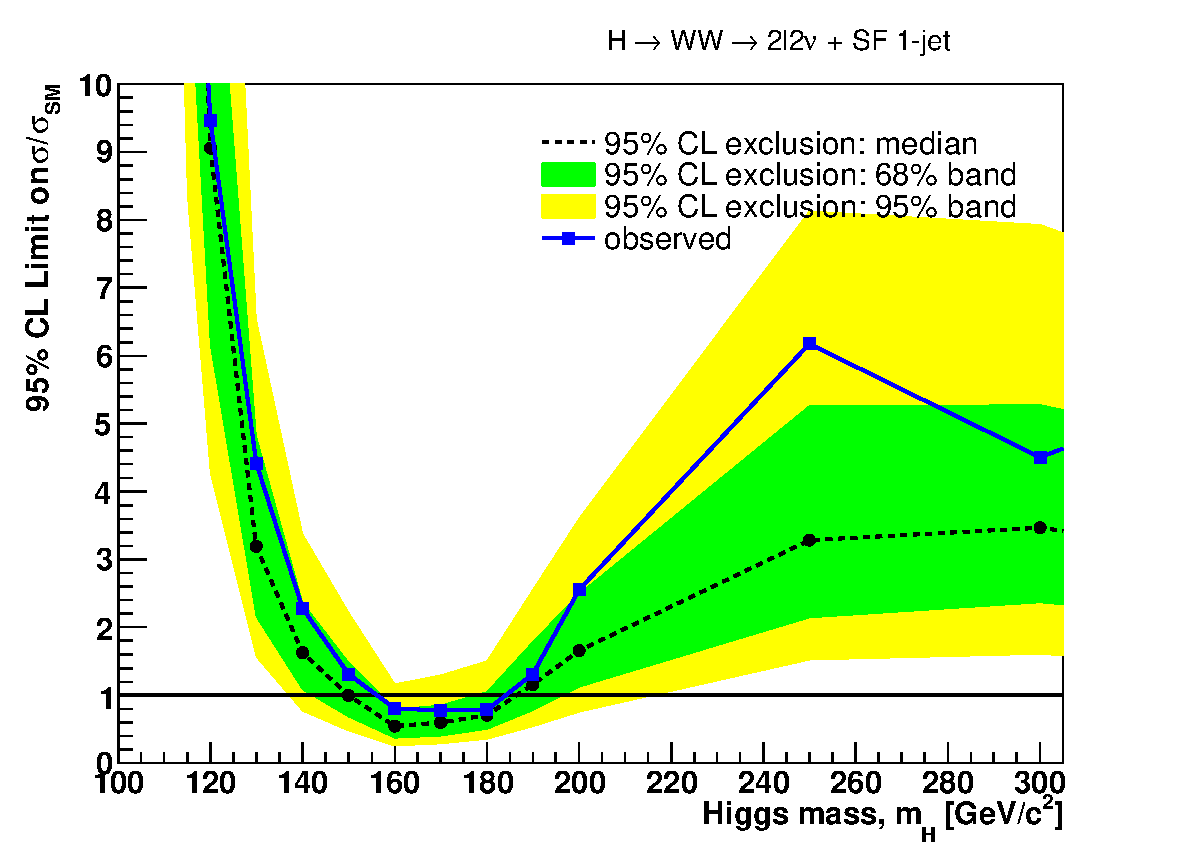
\includegraphics[width=0.49\textwidth]{eps_final/limits_sf_1j_shape.pdf}
   \caption{Shape based analysis upper limits at 95\% C.L. for \usedLumi of data. 
     Left - opposite flavor, right - same flavor }
\end{center}
\end{figure}
\end{document}